\documentclass[a4paper,10pt]{article}
\usepackage[utf8]{inputenc}
\usepackage{amssymb}
\usepackage{amsfonts}
\usepackage{amsmath}
\usepackage{enumerate}
\setlength{\parindent}{0pt}
\usepackage[margin=1in]{geometry}

\usepackage{graphicx}
\graphicspath{ {./images/} }

\usepackage{listings}
\usepackage{color}

\definecolor{dkgreen}{rgb}{0,0.6,0}
\definecolor{gray}{rgb}{0.5,0.5,0.5}
\definecolor{mauve}{rgb}{0.58,0,0.82}

\lstset{frame=tb,
  language=C,
  aboveskip=3mm,
  belowskip=3mm,
  showstringspaces=false,
  columns=flexible,
  basicstyle={\small\ttfamily},
  numbers=none,
  numberstyle=\tiny\color{gray},
  keywordstyle=\color{blue},
  commentstyle=\color{dkgreen},
  stringstyle=\color{mauve},
  breaklines=true,
  breakatwhitespace=true,
  tabsize=3
}
\begin{document}

Jason Qiu

CS 385 Lab $\#14$

\emph{I pledge my honor that I have abided by the Stevens Honor System.}

\begin{enumerate}[1.]
	\item \begin{enumerate}[(a)]
		\item Edges: BE, DE, BD, AB
		\item Weight: 11
		\item Final tree:
		
		\centerline{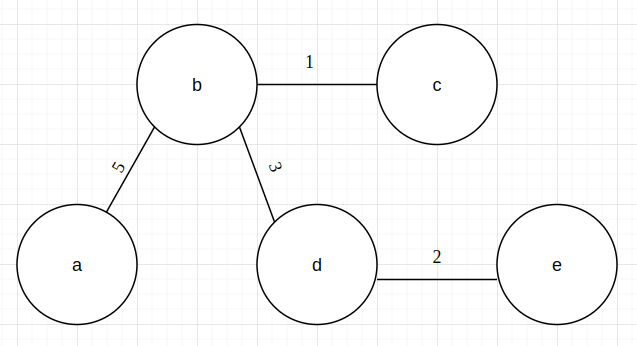
\includegraphics[scale=0.5]{fig1}}	
	\end{enumerate}
	\item Path: $A \rightarrow B \rightarrow C \rightarrow E \rightarrow F$
	
	Distance: 8
	
	\begin{tabular}{|c|c|}
	\hline
	\textbf{Tree Vertices} & \textbf{Remaining Vertices} \\
	\hline
	$a(-, 0)$ & $b(a, 1), c(a, 3), d(-, \infty), e(-, \infty), f(a, 10), g(-, \infty)$\\
	\hline
	$b(a, 1)$ & $c(b, 2), d(b, 8), e(b, 6), f(a, 10), g(b, 3)$\\
	\hline
	$c(b, 2)$ & $d(b, 8), e(c, 5), f(a, 10), g(b, 3)$\\
	\hline
	$g(b, 3)$ & $d(b, 8), e(c, 5), f(a, 10)$\\
	\hline
	$e(c, 5)$ & $d(e, 7), f(e, 7)$\\
	\hline
	$d(e, 7)$ & $f(e, 7)$\\
	\hline
	$f(e, 7)$ & \\
	\hline
	\end{tabular}
	
	\item \begin{enumerate}[(a)]
		\item \ 
		
		\centerline{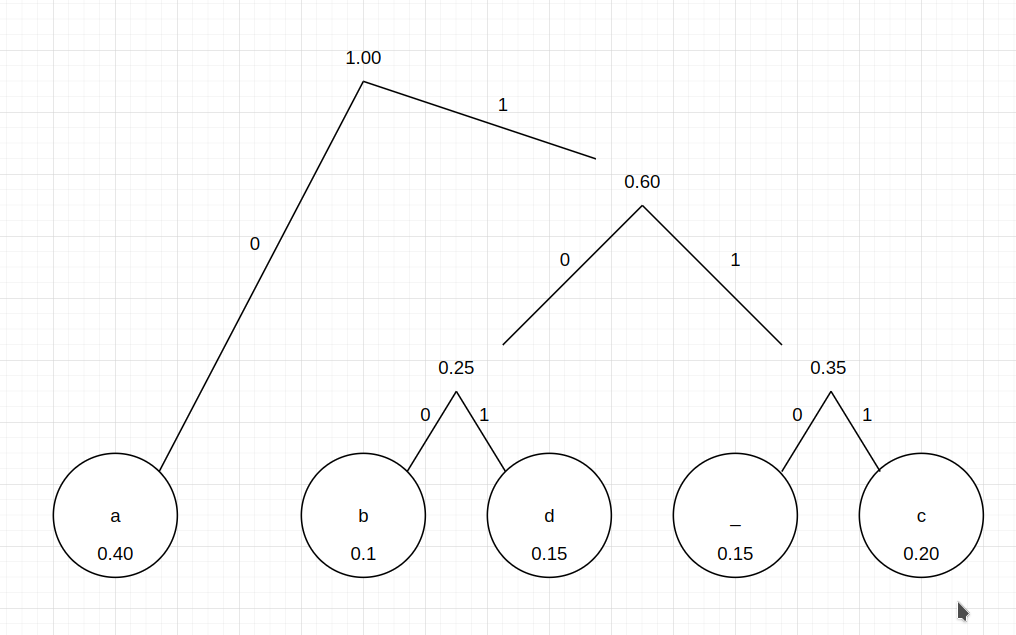
\includegraphics[scale=0.25]{fig2}}
		
		\item 0100011101000101
		\item BAD\_ADA
		\item $$\text{compression ratio} = \frac{3 - \sum_{i} f_i \cdot l_i}{3} = \frac{0.4 \cdot 1 + 0.6 \cdot 3}{3} = \frac{3 - 2.2}{3} \approx 0.267 = \boxed{26.7\%}$$
	\end{enumerate}
\end{enumerate}
\end{document}